\section{Gdev Ecosystem}
\label{sec:overview}

\begin{figure}[t]
 \begin{center}
  %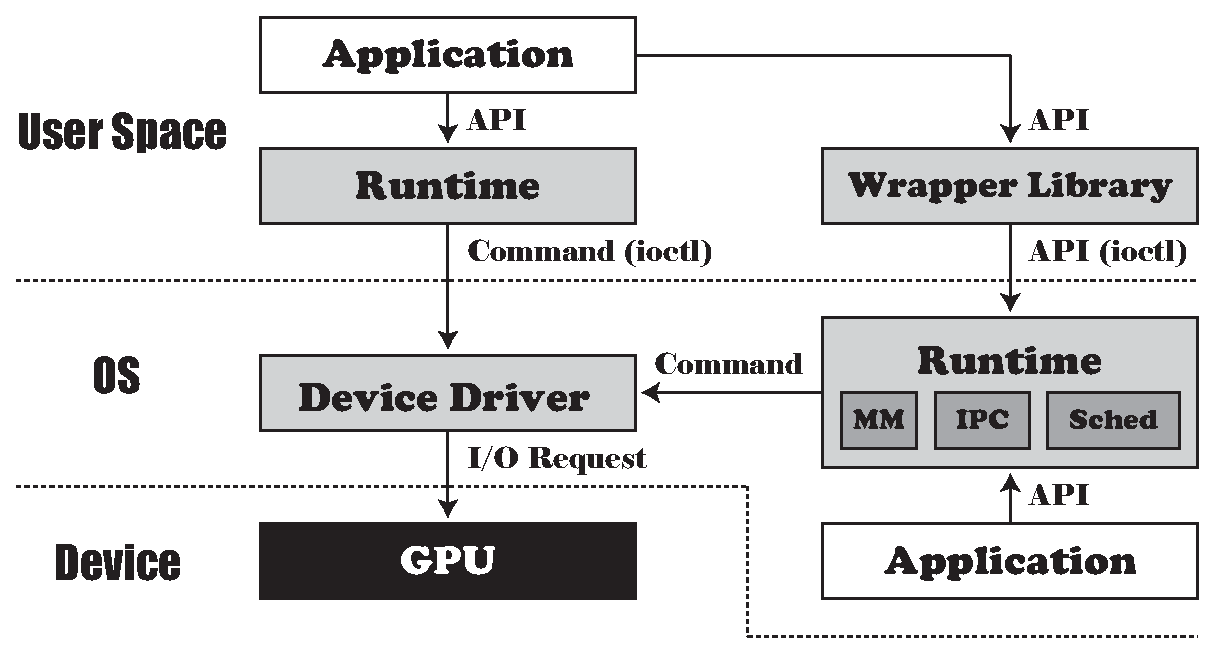
\includegraphics[width=\hsize]{eps/gdev.eps}\\
  \caption{Outline of the Gdev ecosystem.}
  \label{fig:gdev}
 \end{center}
 \vspace{-1em}
\end{figure}

Gdev is aimed at extending GPU resource management capabilities and a
class of applications that can benefit from the GPU.
To this end, it integrates runtime support into the OS.
Figure~\ref{fig:gdev} illustrates the outline of the Gdev ecosystem.
First of all, Gdev still supports a traditional execution model, where
applications call the user-space runtime library through the API, and
the library sends a series of GPU commands to the device driver through
the system call.
As demonstrated in previous work~\cite{Kato_ATC11}, however, it is hard
to analyze what the sequence of GPU commands means at runtime by
software (there could be hundreds of commands for one operation).
It would not therefore be appropriate to call resource management
primitives along with command calls but with API calls.
This argument motives the Gdev design below.

Unlike traditional GPGPU approaches, Gdev employs a runtime engine in
the OS, which composes a set of GPU resource management primitives.
OS applications can directly access this runtime.
User-space applications can also use it through the wrapper library provided by
Gdev, which simply relays API calls to the OS runtime through the system
call.
The GPU resource management of Gdev is API-driven; specifically, Gdev
manages GPU resources upon corresponding API calls.

\subsection{Low-Level API}
\label{sec:low_level_api}

\begin{table}[t]
 \caption{Representatives of Gdev API.}
 \label{tab:gdev_api}
 \begin{center}
  {\footnotesize
  \begin{tabular}{|l|l|}
   \hline
   \textbf{API name} & \textbf{Description}\\
   \hline
   \texttt{gopen}, \texttt{gclose} & Open/close the device\\
   \hline
   \texttt{gmalloc}, \texttt{gfree} & Allocate/free device memory\\
   \hline
   \texttt{gmalloc\_dma}, \texttt{gfree\_dma} & Allocate/free host I/O memory\\
   \hline
   \texttt{gmemcpy\_to\_device} & Copy memory to the device\\
   \hline
   \texttt{gmemcpy\_from\_device} & Copy memory from the device\\
   \hline
   \texttt{glaunch}, \texttt{gsync} & Launch/wait computation\\
   \hline
   \texttt{gquery} & Query device information\\
   \hline
   \texttt{gshmget}, \texttt{gshmctl} & Manage shared device memory\\
   \hline
   \texttt{gshmat}, \texttt{gshmdt} & Share/unshare device memory\\
   \hline
  \end{tabular}
  }
 \end{center}
\vspace{-1em}
\end{table}

Gdev provides a set of low-level API functions for GPU programming as
shown in Table~\ref{tab:gdev_api}.
Programmers can use either the Gdev API or a high-level API, such as
CUDA, internally wrapping the Gdev API.
In either case, the Gdev API functions are eventually used to access
the GPU.
There are several more API functions supported by Gdev, such as
asynchronous memory copy functions, but are not focused on in this
paper.

Table~\ref{tab:gdev_api} shows an initial version of Gdev API.
For now, Gdev API does not support texture memory and 2-D/3-D memory
transfers.
Although this is a current limitation on our prototype implementation,
it is not a conceptual limitation of Gdev.
We believe that the Gdev resource management presented in this paper is
also applicable to those extensions once the API is supported.

\subsection{CUDA Support}

In addition to the low-level API, we provide a limited set of common
CUDA 4.0 Driver API so that legacy CUDA applications can run on top of
Gdev.
The supported API functions are limited to those that can be implemented
by the current version of Gdev API, but many legacy CUDA applications
can perform with such limitations, as we will demonstrate in
Section~\ref{evaluation}.

Our runtime library parses the CUBIN format file.

\subsection{Portability}

\subsection{Open-Source Implementation}

